\section{Conclusions}

\begin{frame}[plain]
  \begin{tikzpicture}[remember picture,overlay]
    \node[at=(current page.center)] {
      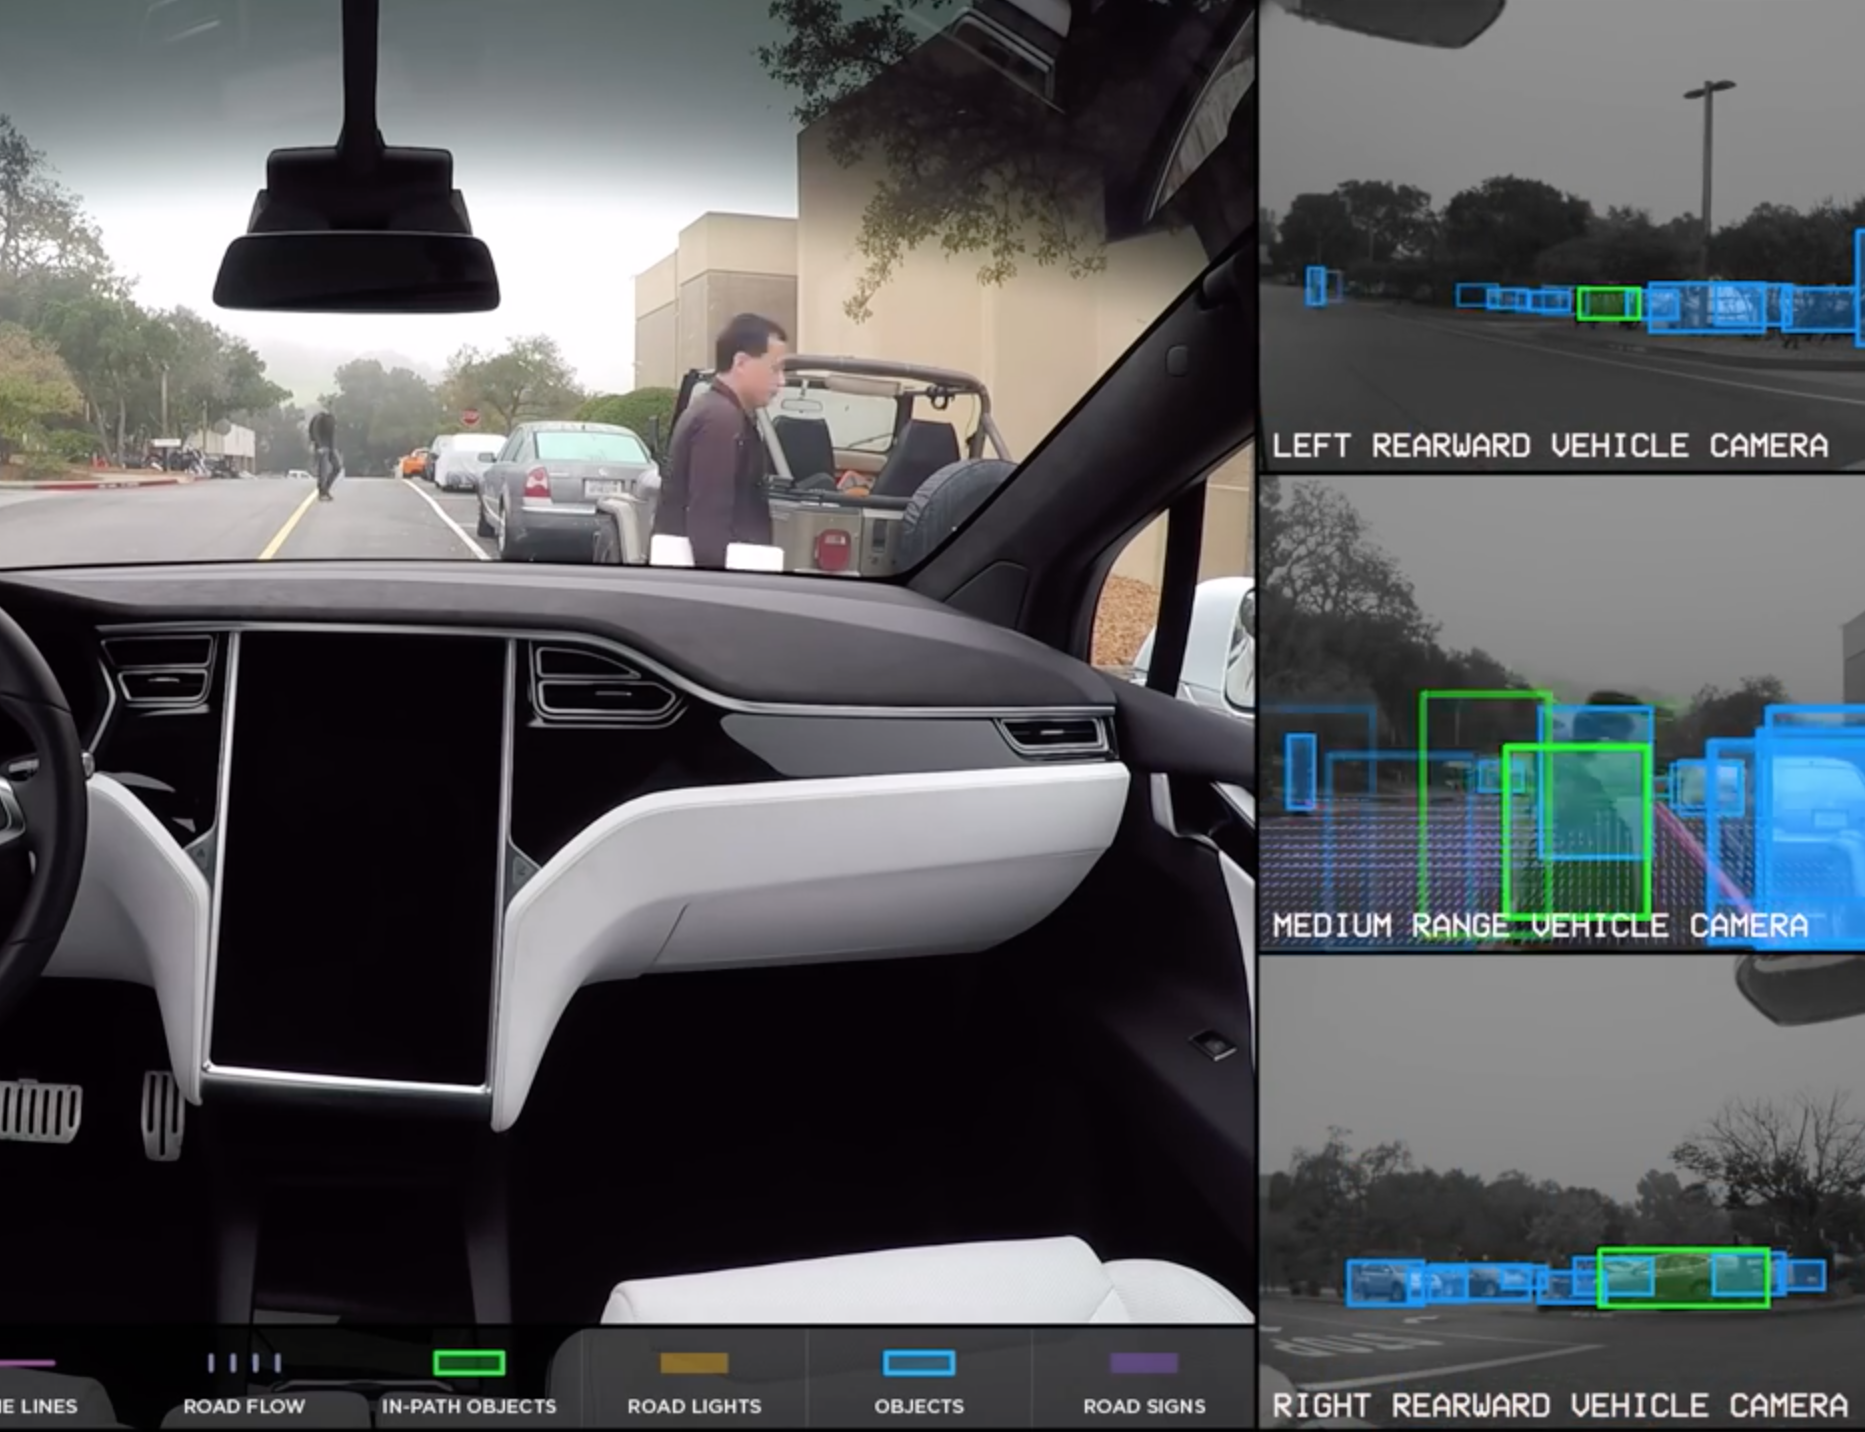
\includegraphics[width=\paperwidth]{intro_tesla.png}
    };
  \end{tikzpicture}
\end{frame}

\begin{frame}{Conclusions}
  \metroset{block=fill}
  \begin{exampleblock}{What have we seen so far?}
    Different methods for pedestrain detection capable of distinguish an human
    in a real world scenario.
  \end{exampleblock}
\pause
  \begin{alertblock}{Are these result good enough?}
    \centering\huge NO
  \end{alertblock}
  \pause
    \begin{alertblock}{Why?}
      High miss rate (15\% to 25\%) and difficulties on real-time implementations
    \end{alertblock}
\end{frame}

\begin{frame}[standout]
  \huge Questions?
\end{frame}


\begin{frame}[allowframebreaks] %allow to expand references to multiple frames (slides)

\frametitle{Bibliography}
\small
\scriptsize{\bibliographystyle{acm}}
\scriptsize
\bibliography{Bibliography} %bibtex file name without .bib extension
\nocite{*}
\end{frame}
